\chapter{Evaluation}\label{C:eval}

\section{Mechanical Stability}
Perform Motor driving parameter sweep to optimise mechanical performance according to requirements; 
of minimising pipette tip overshoot and settling time.
\subsection{Procedure}
\begin{itemize}
    \item Position tip at -1/4 revolution before zero point
    \item Set Speed/acceleration values
    \item Swing to zero position
    \item Repeat for value sleep=1rev/s, acc=1/rev/s/s $\rightarrow$  speed=2rev/s, acc=10/rev/s/s
    \item Note: acceleration is the ramp down at end/start of motion so is what we care most about
    \item Camera captured motion 
\end{itemize}



\subsection{Results}

//insert generated figures of tip position

//generated trend lines/aggregated data (settle, overshoot) from data.
\begin{figure}
    \centering
    \includegraphics[width=0.4\textwidth]{{example-image}}
\end{figure}

\section{Droplet Volume}
Something the previous system could not achieve was dispensing a variety of volumes.
Use e-pipettes programmable volume to investigate the limits of this project.
\begin{itemize}
    \item How large a droplet can be held on to? (prelim: 8uL)
    \item How large (over above) can reliably self release (w/out touch down)
    \item How small a droplet can be dispensed (e-pipette has draw-back).
\end{itemize}    

\begin{center}
    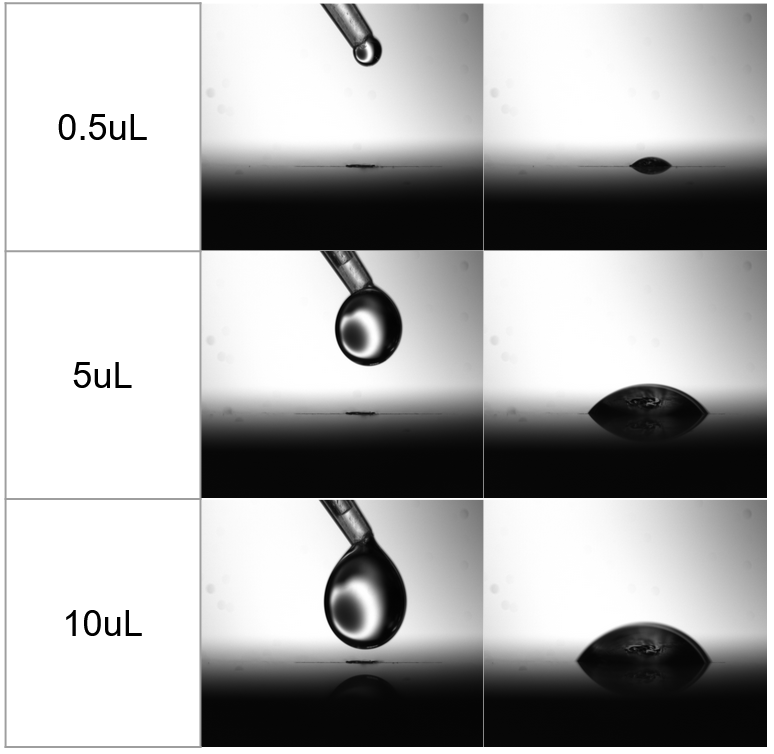
\includegraphics[width=0.4\textwidth]{img/volume_range.png}
\end{center}

\section{Repeatability and Reliability}

This section aims to produce the main set of comparable results for evaluating the projects produced system against the output of the previous setup. Thus justifying the success of one of main goals.

\subsection{Procedure}
\begin{itemize}
    \item \textbf{Initial Setup:} Roughly Position substrate stage, reservoir platform and note angular positions as well as vertical clearance requirements.
    \item \textbf{Zero System:} Using overhead camera precisely position pipette tip above substrate centre
    \item \textbf{Data Acquisition:} Initialise cameras, collect pixel:mm calibration data for analysis, initial LabView temperature logger, and environmental monitor noted. Info: temperature data rate, camera frame rate
    \item \textbf{Automated Sequence:} Via the serial link, enter the procedures command sequence to represent $\rightarrow$ lower, draw up fluid, raise, position over substrate, dispense, lower, raise, clear camera view. With appropriate delays.
    \item \textbf{Capture:} Begin data collection and automated dispense.
    \item \textbf{Repeat: } Minimum of 5 times. Each time carefully cleaning substrate surface to minimised up measured factors. 
\end{itemize}

\newpage
\subsection{Analysis and Results}

To show the system successfully increases the consistency of droplet position and investigate whether this supports the hypothesis that this resulted in better temperature consistency.

\begin{figure}[h]
    \centering
    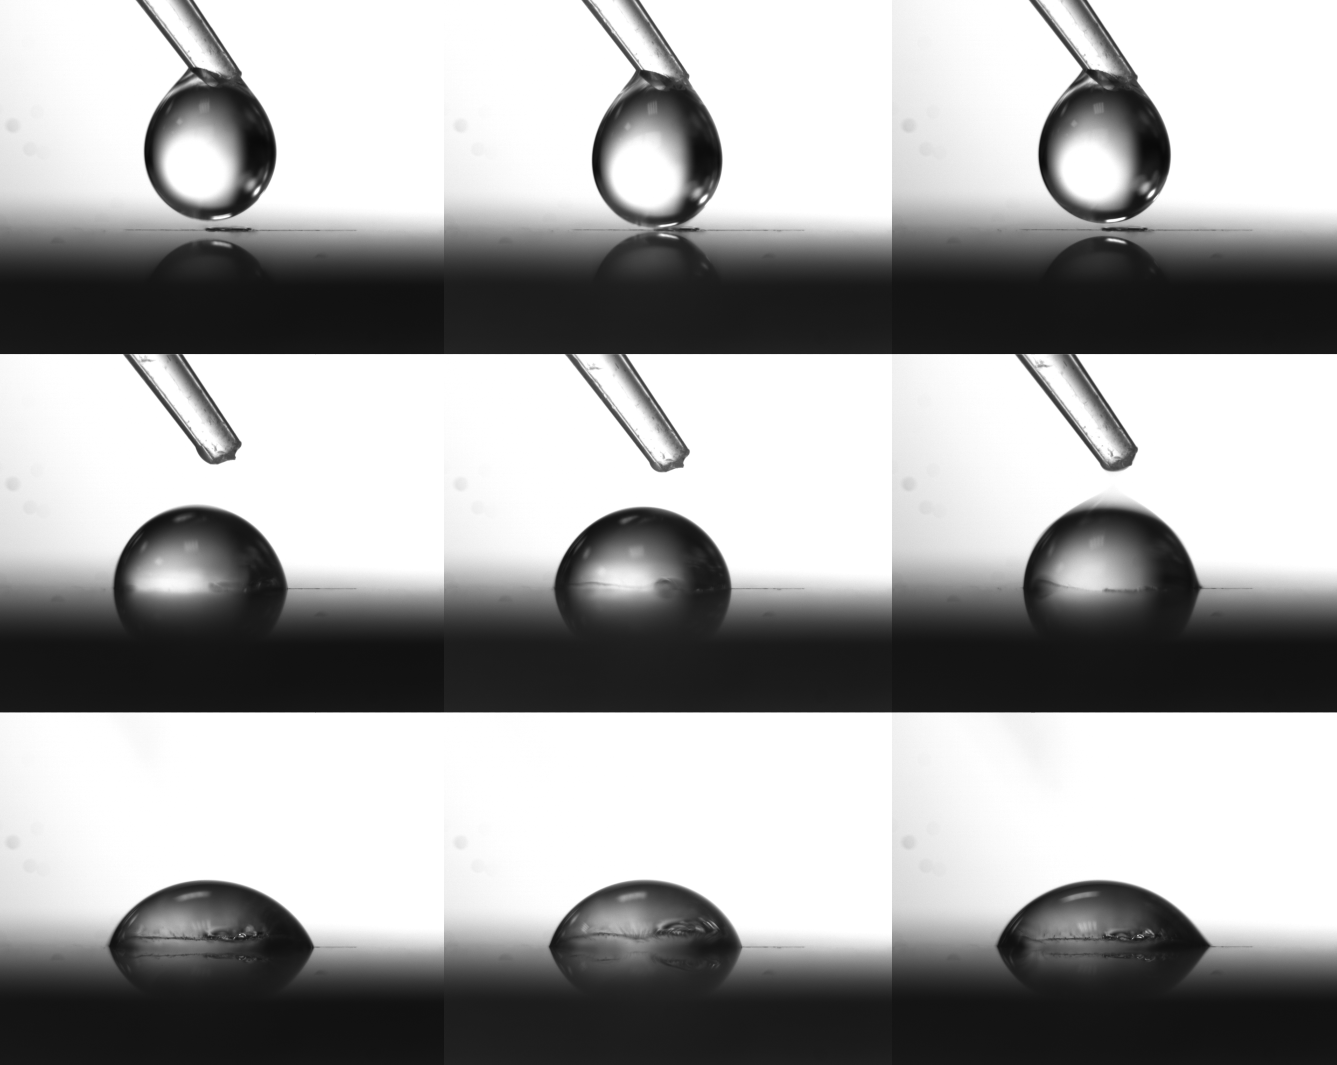
\includegraphics[width=0.4\textwidth]{img/side_drops.png}
    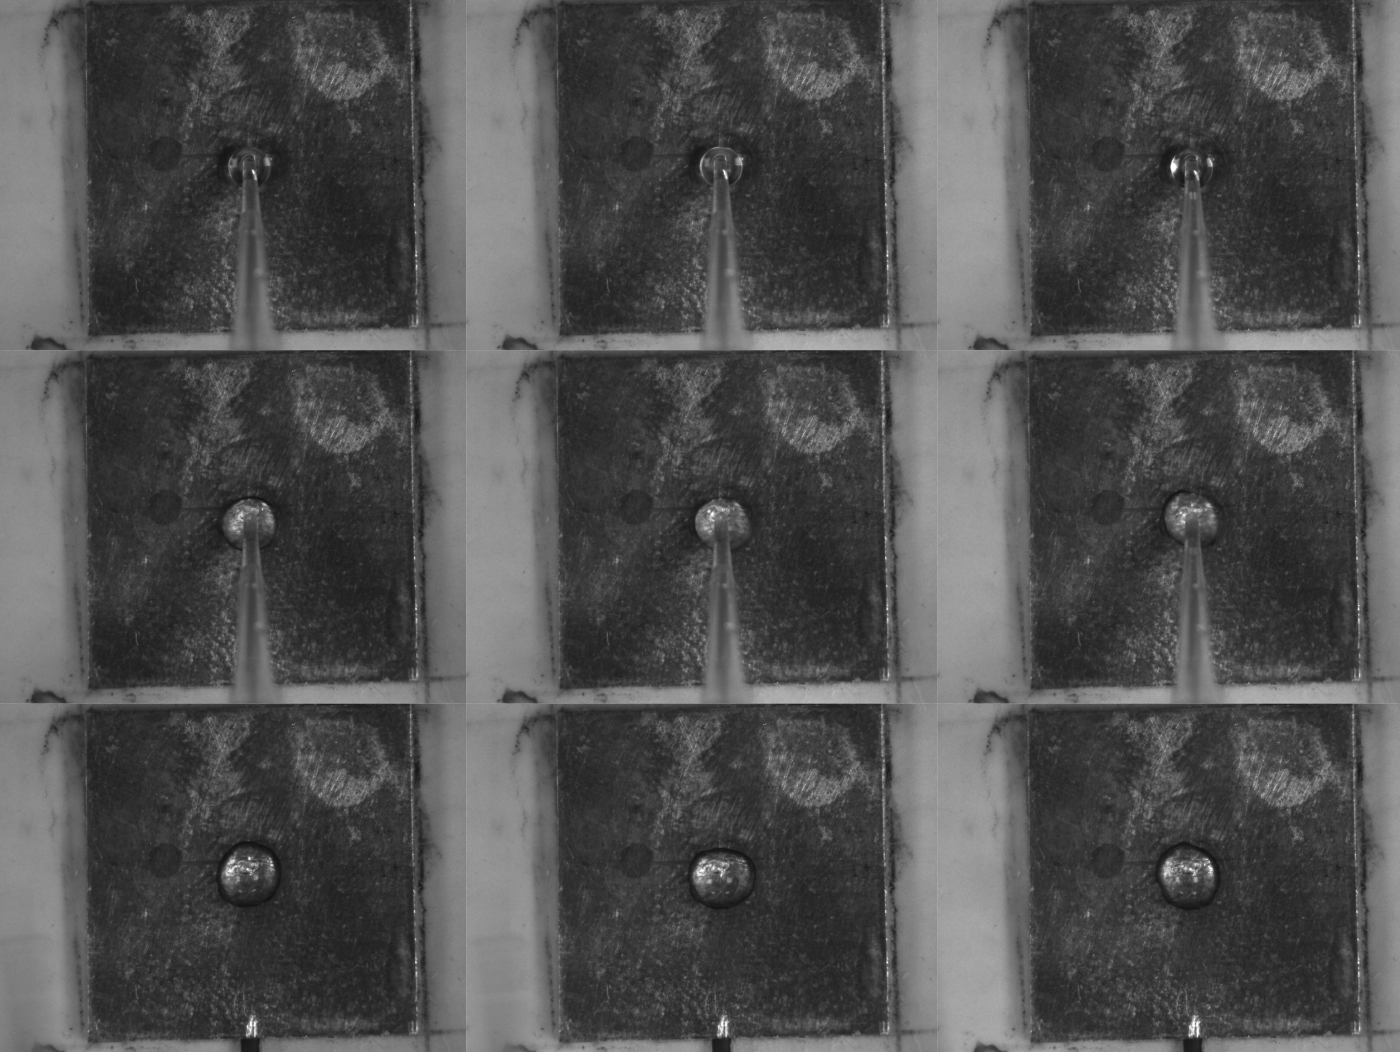
\includegraphics[width=0.4\textwidth]{img/top_drops.png}
\end{figure}

\begin{figure}[h]
    \centering
    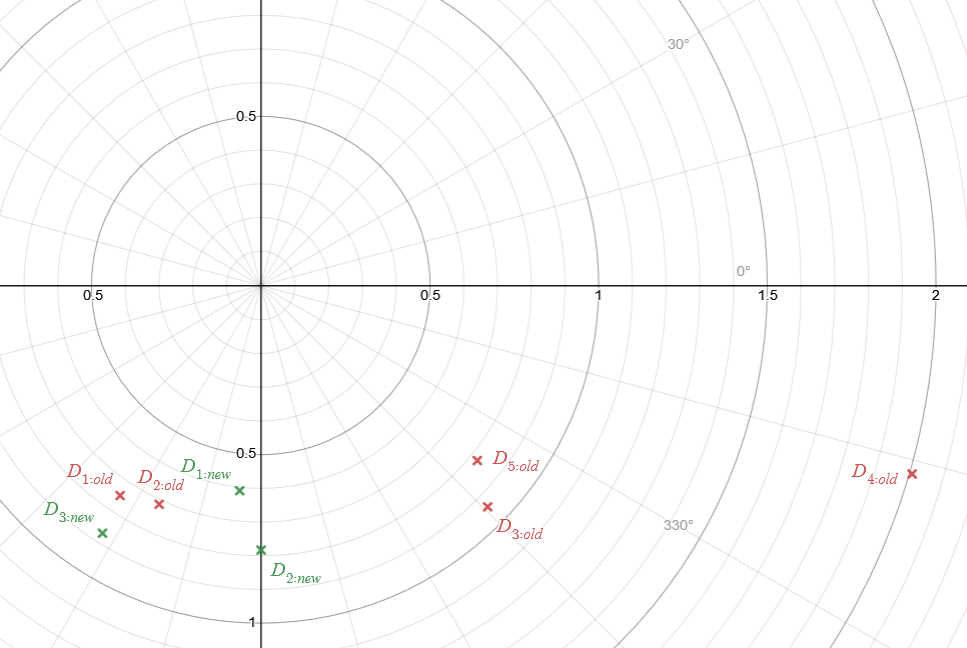
\includegraphics[width=0.4\textwidth]{img/pos_comp.png}
    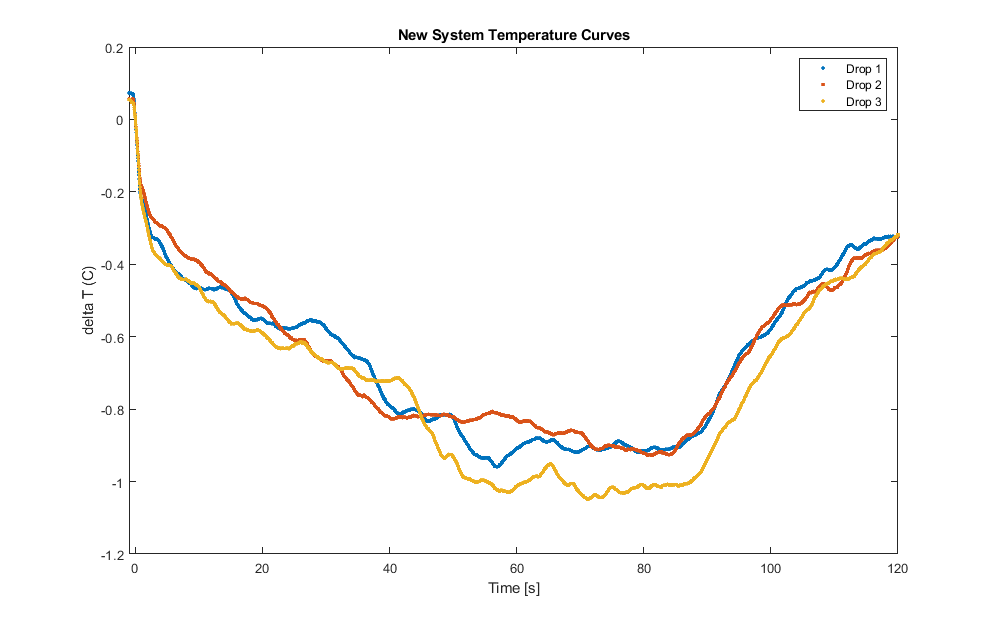
\includegraphics[width=0.4\textwidth]{img/new_temp.png}
\end{figure}

